
\chapter{Integration}
\label{integration_cha}
\authorsection{\editorjulian}
\todo[inline]{Julian: Schreiben}

\section{Aufgabenstellung}
\label{aufgabenstellung_integration_sec}

Die Aufgaben im Bereich der Integration lassen sich unter folgende Punkte einordnen:

\begin{description}
\item[Code Zusammenführen]
Um das Auseinanderdriften der einzelnen Teilprojekte zu vermeiden ist ein regelmäßiges Zusammenführen 
mittels Git notwendig. Zusätzlich ist die Integration von Code der außerhalb des SegwayOmni-Projektes 
entsteht, wie etwa der Kinect-Teil, notwendig. Weiterhin muss die Kompatibilität der Schnittstellen 
zwischen den Teilprojekten gepflegt werden.

\item[Architektur]
Das bestehende hierarchische Grundkonzept muss erweitert werden um eine sinnvolle Kontrolle der 
einzelnen Funktionen des Roboters zu ermöglichen.

\item[Benutzerschnittstelle]
Zur Kontrolle des Roboters durch Benutzer muss eine Benutzerschnittstelle implementiert werden die es 
erlaubt die einzelnen Funktionen der Software zu aktivieren.

\end{description}

\section{Umsetzung}
\label{umsetzung_integration_sec}

\subsection{Architektur}
\label{integration_architektur_sec}

Die Gruppen \lstinline{SegwayOmniBehaviours} und \lstinline{SegwayOmniKinect} verfügen über 
verschiedene Funktionen und bieten wichtige Informationen über den Zustand des Roboters und 
seiner Umwelt. Um diese Informationen sinnvoll verarbeiten zu können und ein Abrufen der einzelnen 
Funktionen zu ermöglichen, ist es notwendig eine Architektur bereitzustellen die dies ermöglicht.

\subsubsection{Hierarchische Struktur}
\label{integration_umsetzung_hierarchie_sec}

In den existierenden Projekten \lstinline{Odete} und \lstinline{SegwayOmni} gab es bereits eine Hierarchie 
in den verwendeten Gruppen, bei der Schritt für Schritt die Abstraktion von der verwendeten 
Plattform bzw. Hardware erfolgte. Diese Hierachie wurde beibehalten und kann in drei Ebenen unterteilt 
werden (siehe \ref{bahnplanung_umsetzung_sec}). Auf der obersten Ebene, der Verhaltensebene, befinden sich die 
Gruppen \lstinline{SegwayOmniBehaviours} und \lstinline{SegwayOmniKinect}. Zur Kontrolle des Roboters kommt 
eine zusätzliche Ebene hinzu, die es erlaubt die einzelnen Verhalten zu aktivieren. Diese Ebene arbeitet auf 
Aufgabenbasis und aktiviert das notwendige Verhalten um eine Aufgabe auszuführen. Eine Aufgabe ist 
beispielsweise: Zeige den gespeicherten Pfad einem Menschen. Auf der Verhaltensebene muss nun die entsprechende 
Funktion aktiviert werden. In diesem Beispiel würde die
\lstinline{SegwayOmni-}\lstinline{Kinect}-Gruppe das Verhalten zum Beobachten
eines Menschen ausführen und die \lstinline{SegwayOmni-Behaviours}-Gruppe das
Verhalten zum Abfahren eines gespeicherten Pfades.

Die Funktionen des Roboters können, auf oberster Ebene, in einzelne, unabhängige Aufgaben getrennt werden. Zur Erfüllung dieser Aufgaben müssen wiederum bestimmte Verhalten ausgeführt werden.
\begin{table}[h]
	\label{tab:integration_aufgaben}
	\centering
	\begin{tabular}{|p{3.7cm}|p{3cm}|p{3.2cm}|}
	\hline
	\textbf{Aufgabenebene}	&	\multicolumn{2}{c|}{\textbf{Verhaltensebene}}\\
		&	\textbf{Bahnpl./Steur.}	&	\textbf{Kinect}	\\
	\hline
	Initialisierung	&	Initialisierung	&	Initialisierung \\
	\hline
	Warten auf Person	&	Idle	&	Warten auf Person + Warten auf Geste \\
	\hline
	Warten auf Geste	&	Idle	&	Warten auf Geste \\
	\hline
	Verfolge Person	&	Verfolge Person + Zeichne Pfad auf	&	Tracke Person + Warte auf Geste \\
	\hline
	Kehre zum Start zurück	&	Kehre zum Start zurück	&	Warte auf Geste \\
	\hline
	Zeige Pfad	& Zeige Pfad	&	Tracke Person + Warte auf Geste \\
	\hline
	\end{tabular}
	\caption{Darstellung der Aufgaben und der entsprechenden Verhalten.}
\end{table}
In einem ersten Schritt ist es sinnvoll diese Funktionen zu strukturieren, in dem jeder Aufgabe ein 
interner Zustand zugewiesen wird. Da bei diesem Projekt nicht der Dialog mit dem Roboter sondern lediglich 
die Aktivierung verschiedener Funktionen durch Gesten gewünscht ist, erfolgt der Wechsel der internen 
Zustände durch eine deterministische Zustandsmaschine. Bei komplexeren 
Aufgaben, oder in Szenarien bei der die beobachtete Umwelt nicht deterministisch aufgefasst wird, stößt 
eine einfache Zustandsmaschine an ihre Grenzen und es muss eine Planer verwendet werden.
Neben der globalen Zustandsmaschine im Modul
\lstinline{SegwayOmniStateMode-Manager} erhält jede Gruppe in der darunterliegenden Hierarchieebene (die Verhaltensebene) ebenfalls eine Zustandsmaschine; 
realisiert sind diese in den Modulen \lstinline{SegwayOmniBehavioursManager} bzw. \lstinline{SegwayOmniKinectManager}.

Mit Hilfe dieser hierarchischen Architektur und durch das Arbeiten mit Zuständen kann effizient und für 
den Benutzer stets transparent, die Robotersoftware kontrolliert werden.

\subsubsection{Zusammenspiel der Zustandsmaschinen}
\label{integration_umsetzung_zusammenspiel_sec}

Ein gängiges Konzept zur Steuerung von Robotern bildet 
eine \textit{Sense-Plan-Act-Schleife}\footnote{Dt.: Beobachten-Planen-Handeln-Schleife}, bei der 
ständig die Umwelt sensorisch erfasst und entsprechend der Beobachtung und des aktuellen Zustandes 
eine Handlung ausgeführt wird.
\begin{figure}[h]
	\label{fig:integration_sense_plan_act}
	\centering
	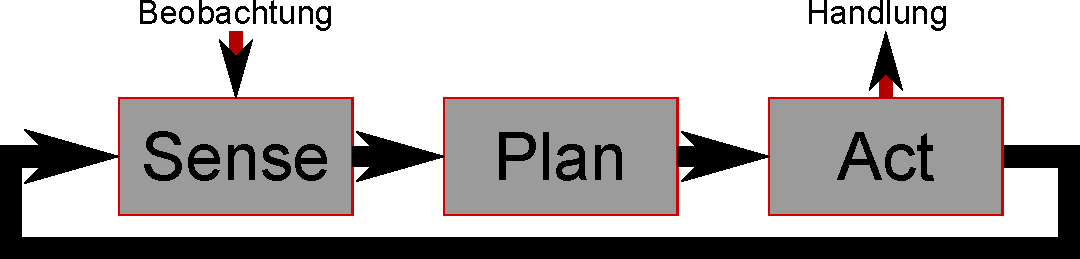
\includegraphics[scale=0.5]{graphics/SCHEMA-SensePlanAct.pdf}
	\caption{Schematische Darstellung des Konzeptes der Sense-Plan-Act-Schleife.}
\end{figure}
Die globale Zustandsmaschine bildet in diesem Konzept das Plan-Modul. Sie erhält von den Gruppen auf 
der Verhaltensebene Informationen, auf Basis derer die Entscheidung für einen Zustandswechsel 
getroffen wird. Ändert sich der Zustand der globalen Zustandsmaschine kann, muss aber nicht, eine 
Handlung folgen. Eine Handlung wird ausgeführt in dem die globale Zustandsmaschine, durch das 
Setzen der entsprechenden Zustände auf Verhaltensebene, ein bestimmtes Verhalten aktiviert oder 
auch ein momentan aktives Verhalten beendet.

Die \lstinline{Mca2}-Architektur bietet, durch die strikte Trennung des Informationsflusses in 
einen \lstinline{Con-trol}- und \lstinline{Sense}-Teil, eine passende Grundlage
für das zuvor beschriebene Konzept. Jede Zustandsmaschine ist in zwei Teile gespalten. Im \lstinline{Sense}-Teil 
erfolgt die Verarbeitung neuer Informationen. Dies geschieht indem, entsprechend dem vorherrschenden 
inneren Zustand und der beobachteten, externen Variable, ein Übergang zu einem neuen Zustand 
ausgeführt wird. Beispielsweise kommt die Ausführung der Aufgabe \textit{Verfolge einen Menschen} 
durch die Geste \textit{Stop} zu ihrem Ende. Im \lstinline{Control}-Teil werden hingegen 
Handlungen ausgeführt. Hier erfolgt, entsprechend dem momentanen inneren Zustand, zum Beispiel 
das Setzen eines neuen Zustandes für in der Hierarchie tiefer liegende Zustandsmaschinen. 
Ein passendes Beispiel ist der Zustand \lstinline{stopFollowing-Person} der
globalen Zustandsmaschine, welcher wiederum den Zustand \lstinline{stopFollowingPerson} im
\lstinline{SegwayOmniBehavioursManager} setzt und so das Beenden des momentanen Verhaltens initialisiert. Erst wenn die aufgezeichnete 
Trajektorie gespeichert und der Roboter gestoppt ist, erfolgt die Rückmeldung, indem die 
Zustandsmaschine in den Zustand \lstinline{idle} wechselt. Dieser neue Zustand wird 
im \lstinline{Sense}-Teil der globalen Zustandsmaschine verarbeitet und falls alle weiteten 
Bedingungen erfüllt sind wird die Aufgabe durch einen letzten Zustandswechsel, ebenfalls in 
den Zustand \lstinline{idle}, beendet (siehe \ref{fig:integration_statemachine}).


\subsection{Benutzerschnittstelle}
\label{benutzerschnittstelle_integration_cha}

Gemäß der Konzeption des Roboters erfolgt die Steuerung vollständig über Gesten. Die Erkennung der Gesten 
geschieht in der Gruppe \lstinline{SegwayOmniKinect}; die Verarbeitung der Gesten im Modul \lstinline{SegwayOmniStateModeManager}. Entsprechend der in Abschnitt \ref{integration_umsetzung_zusammenspiel_sec}
 erläuterten Systematik, entscheidet die globale Zustandsmaschine in jedem Zustand individuell, welche Handlung 
 nach der Beobachtung einer bestimmten Geste folgt. Beim ersten Test der Gestensteuerung hat sich gezeigt, 
 dass eine zuverlässige Steuerung nur durch das Erkennen einer Abfolge mehrerer Gesten möglich. 

Es trat das Problem auf, dass während des Einnehmens einer bestimmten Haltung, die entsprechend der Definition 
der Kinect-Gruppe einer Geste entsprach, regelmäßig eine nicht gewünschte Geste erkannt wurde. Um dieses Problem 
zu lösen kommt eine Steuerung zum Einsatz, bei der nur durch eine Folge von Körperhaltungen eine Geste erkannt 
wird und so eine Funktion auslöst. Bereits bei der Initialisierung einer Person ist es notwendig eine korrekte 
Folge von Haltungen einzunehmen die signalisieren dass man auch wirklich den Roboter steuern möchte. Auch beim Ausführen einer Geste um eine bestimmte Funktion des Roboters, etwa das Abfahren eines Pfades, zu aktivieren, ist es notwendig zuerst eine Anrückhaltung einzunehmen und von dieser zu einer Haltung überzugehen die letztlich die 
Funktion aktiviert.

\begin{landscape}
\begin{figure}
	\label{fig:integration_statemachine}
	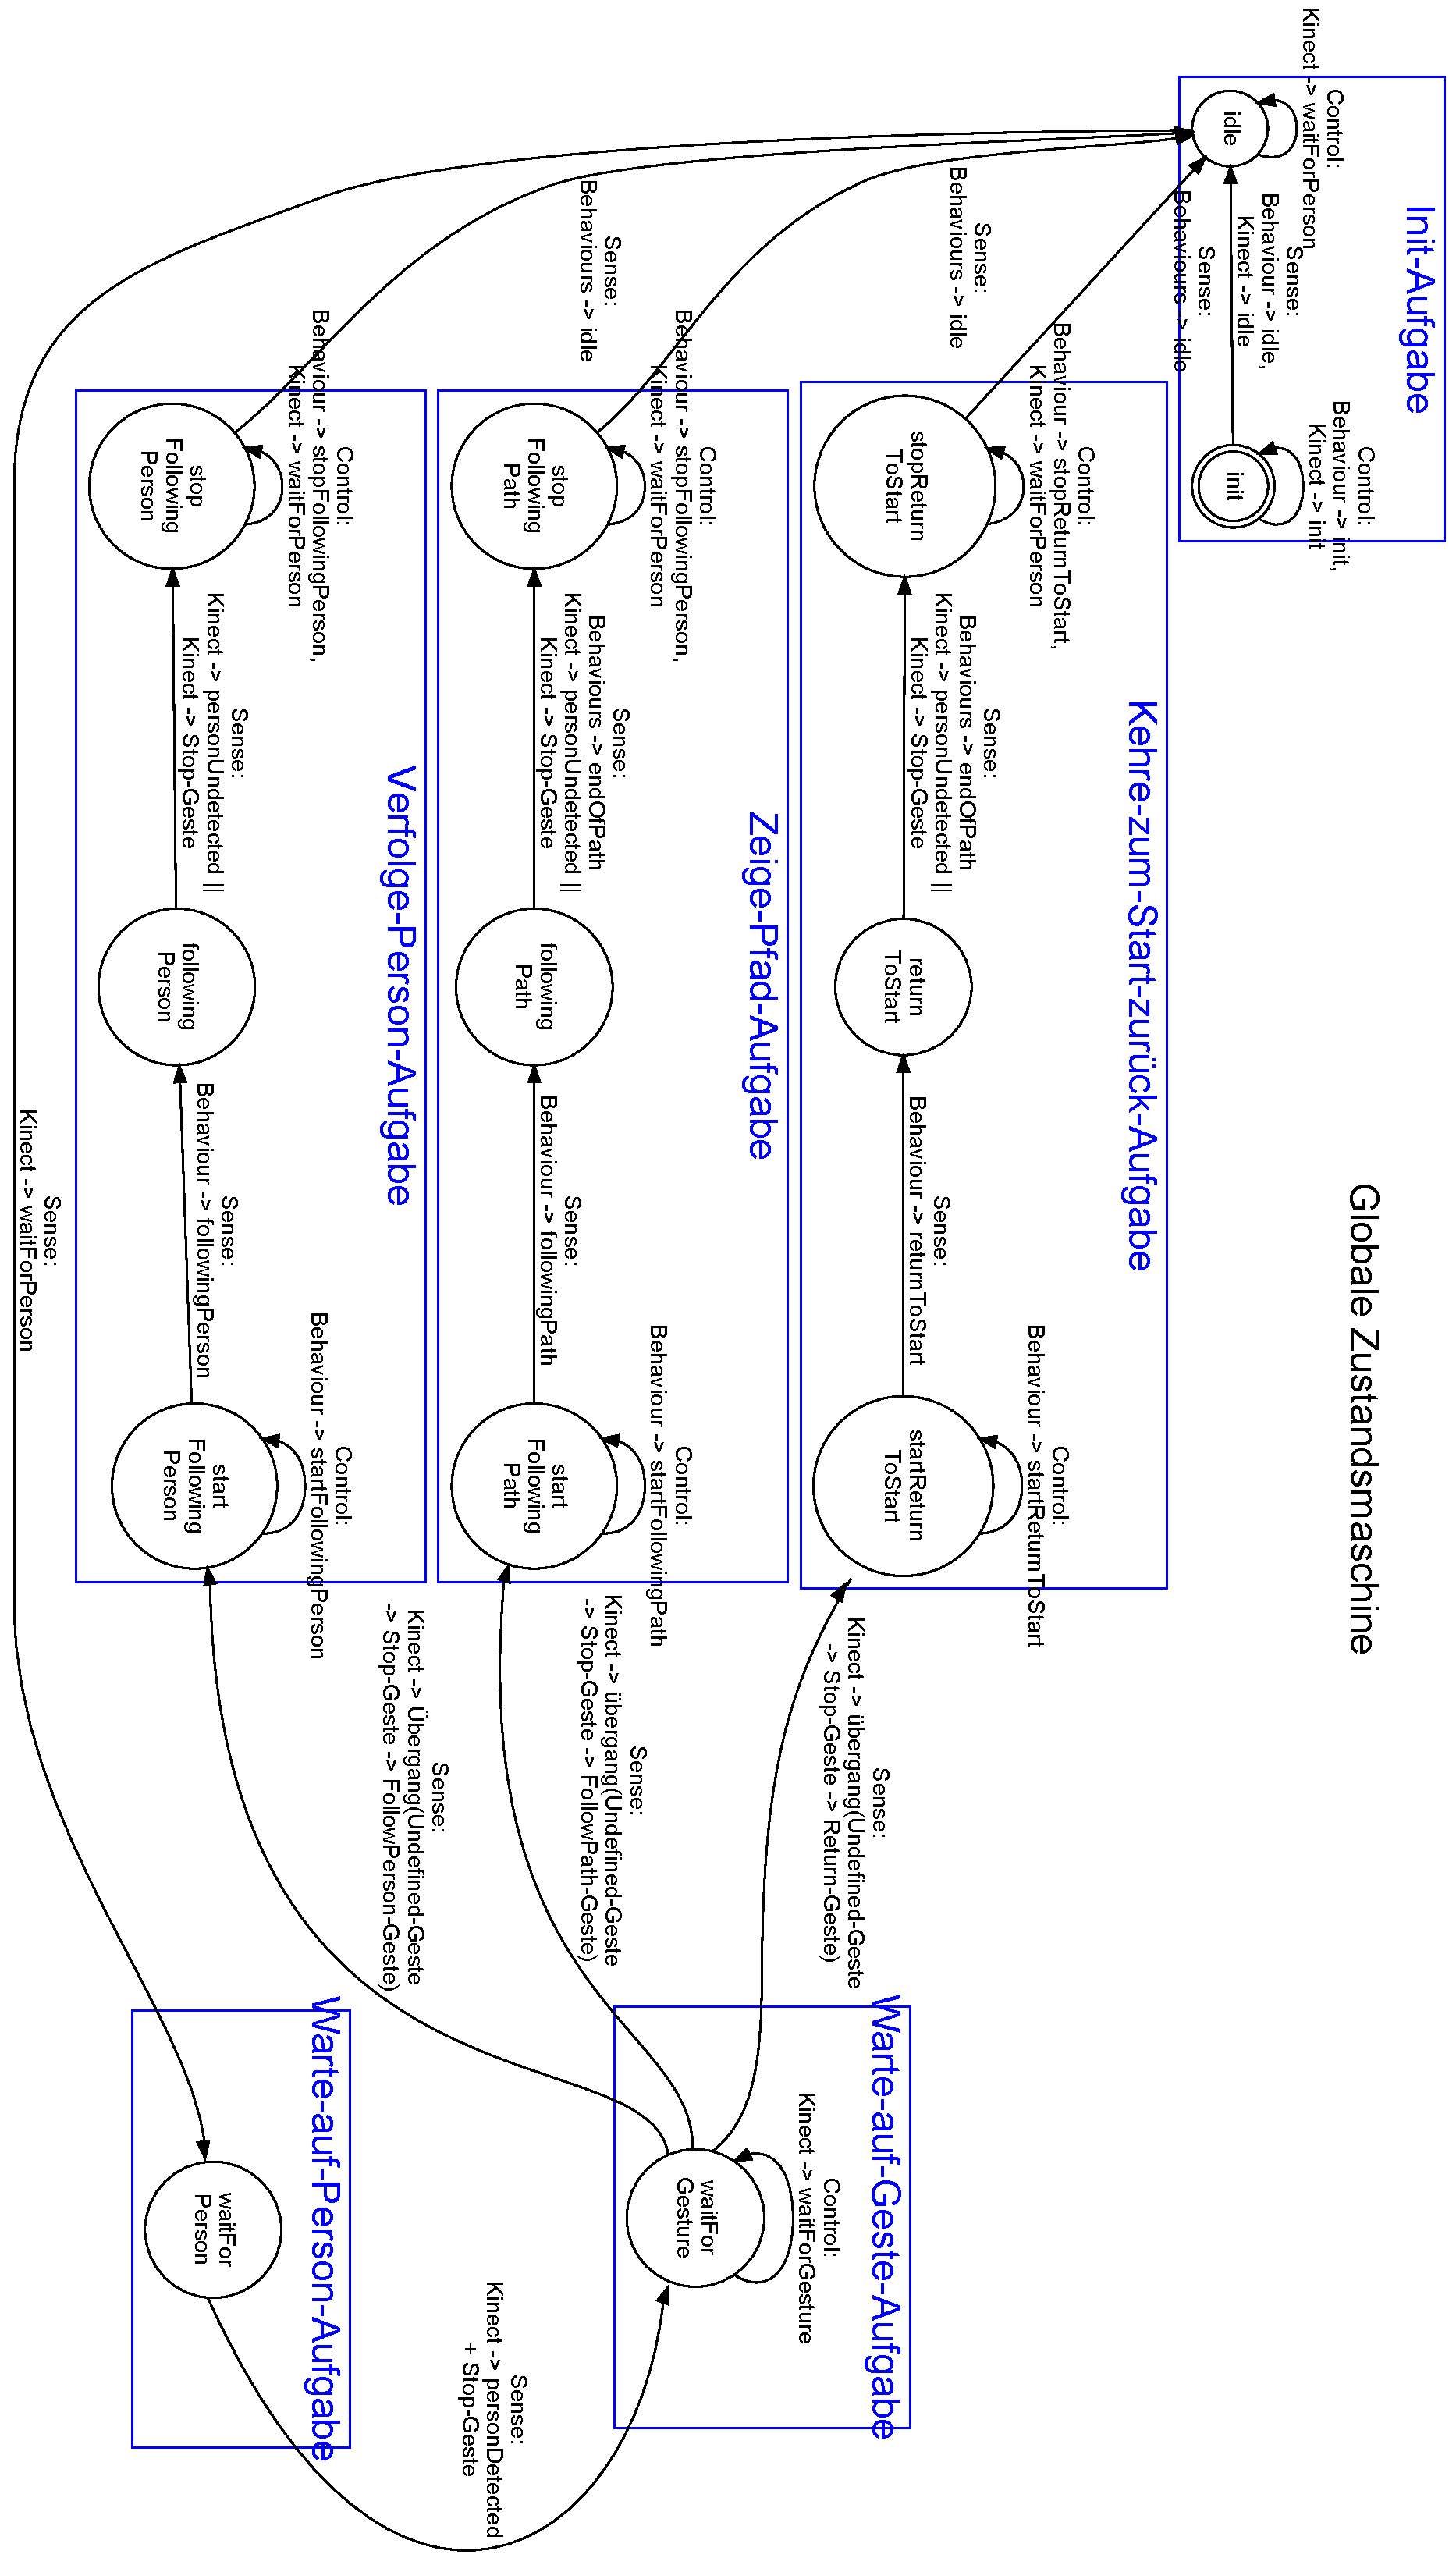
\includegraphics[scale=0.43,angle=90]{graphics/SCHEMA-GlobalStateMachine-hk.pdf}
	\caption{Zustandsdiagramm der globalen Zustandsmaschine}
\end{figure}
\end{landscape}

